\documentclass[\main.tex]{subfiles}


\chapter{Visão Geral}
\begin{singlespace}
\minitoc
\end{singlespace}
\vspace{20pt}

% \section{Tecnologias Utilizadas}
% \subsection{Desenvolvimento da Aplicação}
% ASP.NET, Angular, MS SQL Server (Azure Cloud Database)

% \subsection{Ambiente de Desenvolvimento}
% JetBrains Rider, VSCode, Overleaf

% \subsection{Gestão do Projeto}
% GitLab (issue tracker e wiki's)

\section{Applicação Web}
Na figura 2.1 é possível analisar um diagrama de Casos de Uso relativo à aplicação web de um
modo geral.\par
\begin{figure}[h!]
\centering
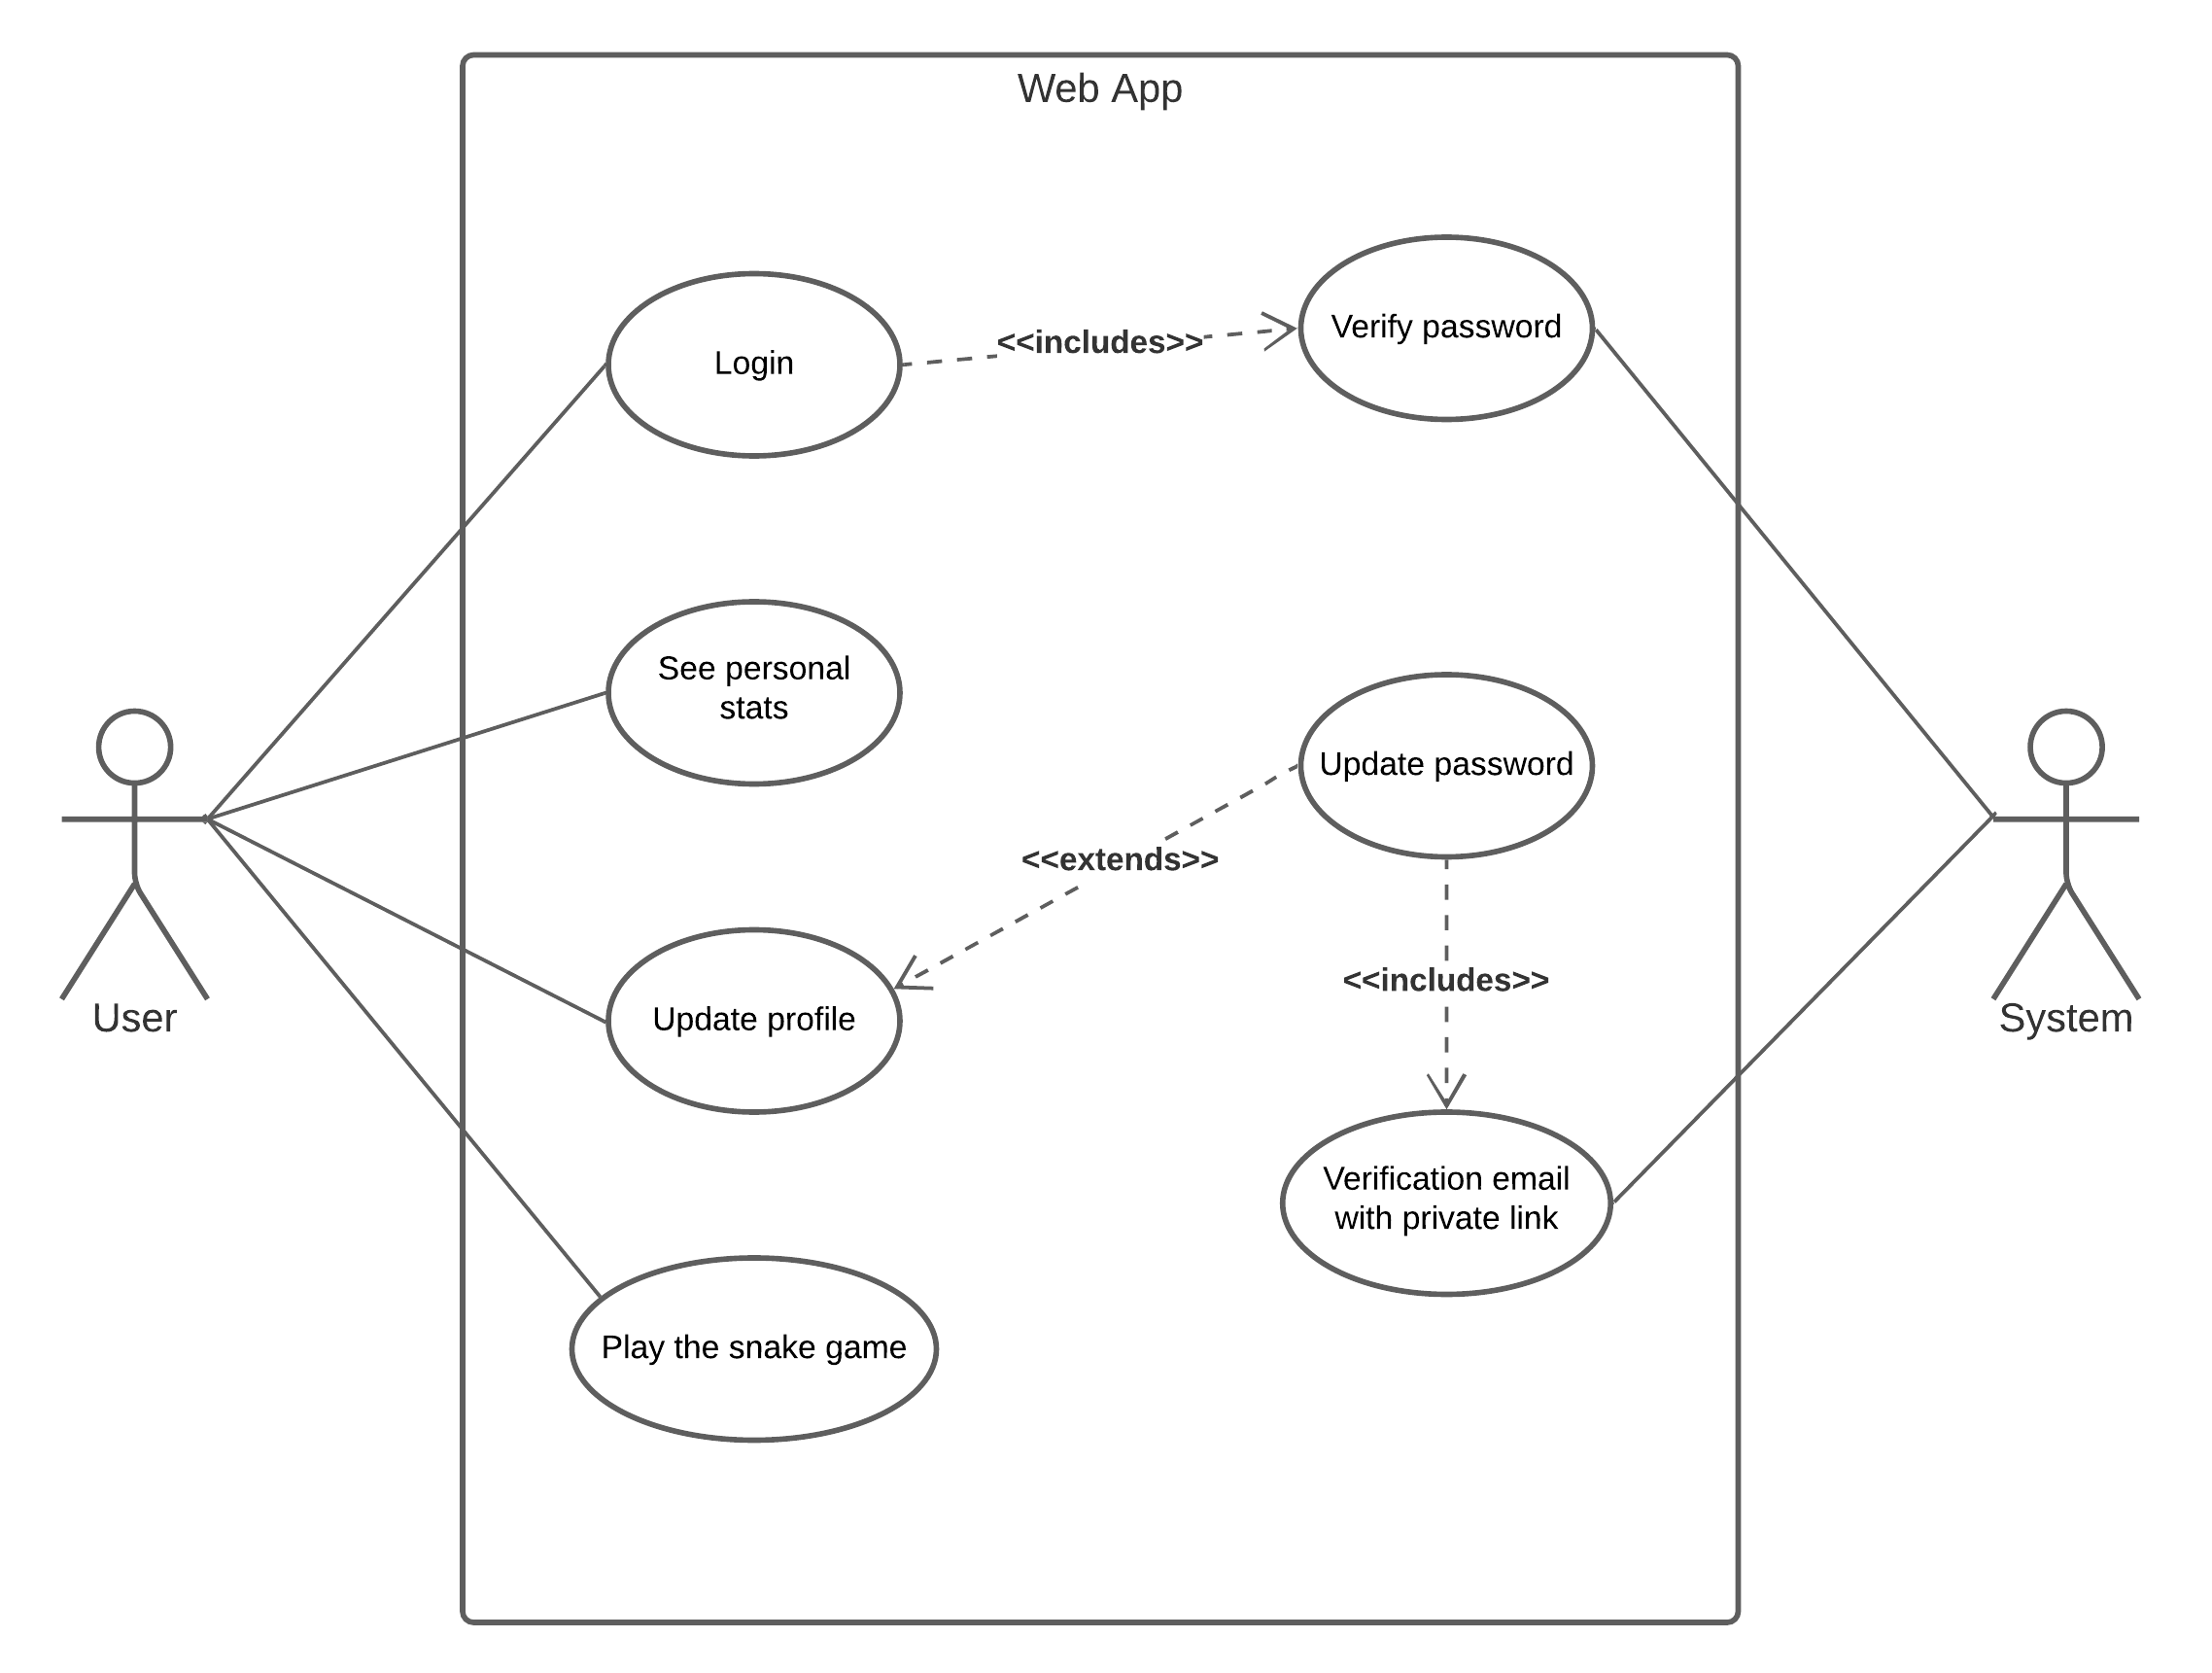
\includegraphics[width=\linewidth]{../private_assets/UML_UseCase_WebApp.png}
\caption{Diagrama de Casos de Uso da Web App}
\end{figure}
\newpage
A aplicação web deve consistir numa plataforma simples e de fácil utilização, por isso a sua
responsividade e usabilidade devem ser muito elevadas. O utilizador deve ser capaz de se
registar e de se autenticar. Com o login realizado, deverá ser capaz de criar ou de se juntar
a uma sessão de jogo para disfrutar do magnifico e único jogo da cobra, mas numa versão mais
competitiva e aliciante. Para além disto, o utilizador poderá ser capaz de visitar a sua página
pessoal com as suas estatísticas de partidas realizadas, bem como ter a possibilidade de
atualizar qualquer dado pessoal introduzido no registo.\par



\section{API REST}
Na figura 2.2 está representado um desenho concetual da arquitetura da API.\par
\begin{figure}[ht]
\centering
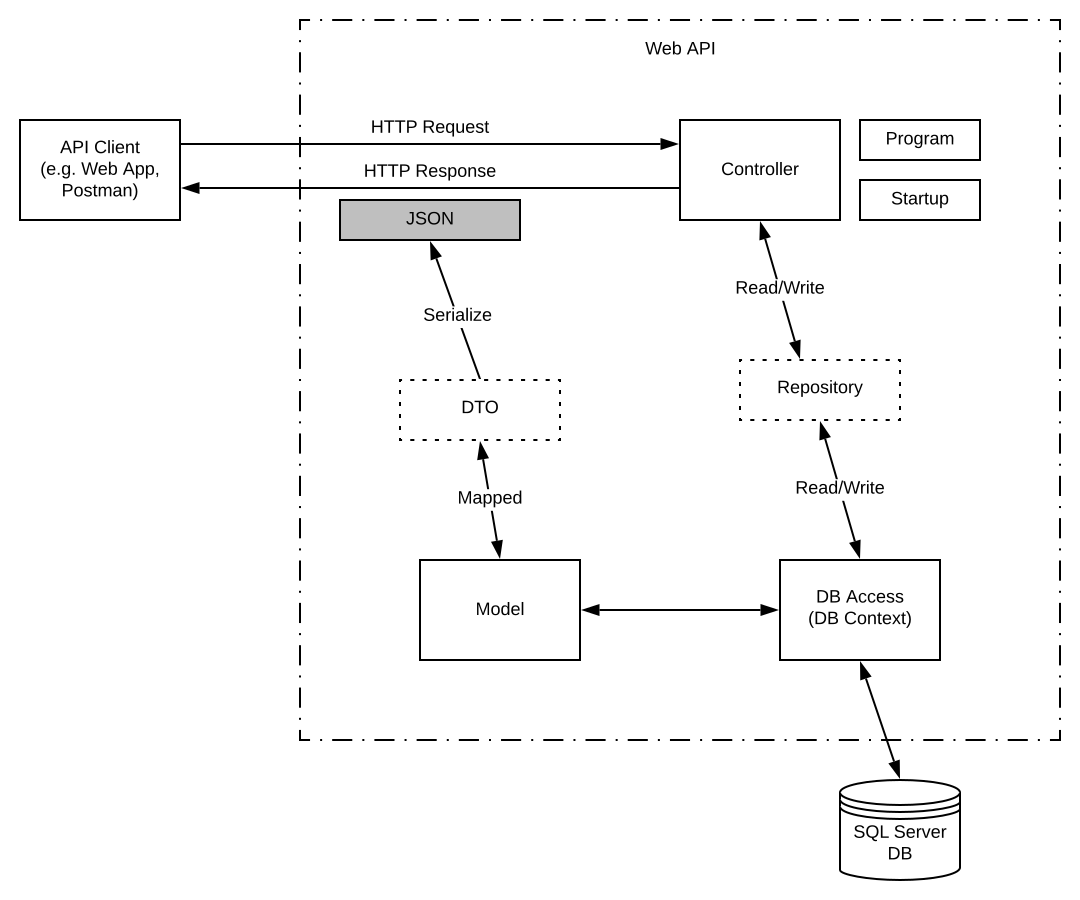
\includegraphics[width=\linewidth]{../private_assets/UML_APIArchitecture.png}
\caption{Arquitetura da API REST}
\end{figure}
A \acrshort{api} será desenvolvida com a utilização do padrão \acrfull{rest}. Para iniciar,
quando é realizado um pedido \acrshort{http} através de um cliente da \acrshort{api} (e.g., a
nossa aplicação web), este é recebido e tratado por um \textit{Controller} que irá comunicar
com a \acrfull{bd} do sistema através do componente \textit{DBContext}. Para que o controlador
consiga comunicar com este componente de forma mais genérica e modularizada será desenvolvido
um componente \textit{Repository}.\par
A informação retornada pela \acrshort{bd} é estruturada pelo \textit{Model} e existirá também
um componente \acrfull{dto} para gerir a informação que deve ser enviada na resposta, de modo a
evitar fugas de informação. Para finalizar, a resposta é enviada num formato \acrshort{json}.
\newpage